\documentclass[10pt,a4paper]{article}
\usepackage[margin=1in]{geometry}
\usepackage{fontspec}
\usepackage{xeCJK}
\usepackage{setspace}
\usepackage{hyperref}
\usepackage{booktabs}
\usepackage{amsmath}
\usepackage{graphicx}
\usepackage{float}

\setstretch{1.0}
\setmainfont{TeX Gyre Termes}
\setCJKmainfont{Noto Serif CJK TC}
\graphicspath{{./}}

\title{\textbf{Final Report: Fast 2D Fluid Dynamics on GPU}\\
\large Reproducing GPU Gems Chapter 38 with CPU--GPU Verification}
\author{第5組\\
112550191 \quad 許書瑋 \qquad 112550052 \quad 林哲安}
\date{\today}

\begin{document}
\maketitle
\thispagestyle{empty}

\begin{abstract}
This report presents the completed implementation of a real-time 2D incompressible fluid simulator based on \textit{GPU Gems} Chapter 38. We provide a CPU reference solver, a CUDA GPU solver, numerical correctness validation, performance benchmarks, and an interactive OpenGL visualization with dye rendering and mouse interaction. Results show strong CPU--GPU agreement and substantial GPU speedup on larger grids.
\end{abstract}

\section{Introduction}
Fluid effects such as smoke and ink are common in games and animation, but solving the underlying physics on a fine grid is expensive. This project reproduces the stable-fluids pipeline from GPU Gems Chapter 38 on modern hardware: simulation runs on the GPU via CUDA, while OpenGL displays the result in real time.

Our objectives were to (1) implement the full simulation pipeline, (2) verify that GPU results match the CPU reference, (3) measure performance across grid sizes and pressure-solver iteration counts, and (4) deliver an interactive demo that makes the flow behavior easy to observe.

\section{Method and Implementation}
\subsection{Simulation Pipeline}
Each timestep follows the stable-fluids sequence (GPU Gems / Stam):
\begin{enumerate}
    \item semi-Lagrangian advection of velocity;
    \item implicit velocity diffusion (viscosity) via Jacobi iteration when \texttt{--viscosity} $> 0$;
    \item external force injection (deterministic center source and mouse input);
    \item advection and sourcing of a passive dye field;
    \item divergence computation;
    \item Jacobi pressure solve;
    \item pressure-gradient projection to enforce near incompressibility.
\end{enumerate}
Default benchmarks and the demo screenshot use \texttt{--viscosity 0} (no diffusion step); diffusion can be enabled for closer alignment with the full Chapter~38 pipeline.

\subsection{CPU and GPU Design}
\begin{itemize}
    \item \textbf{CPU reference}: array-based loops for correctness baseline.
    \item \textbf{GPU solver}: CUDA kernels with one thread per grid cell and double-buffered fields.
    \item \textbf{Visualization}: \texttt{--backend gpu} uses CUDA--OpenGL PBO interop (no per-frame device readback during display); \texttt{--backend cpu} runs the same solver on the CPU and uploads RGBA from host memory for side-by-side performance comparison.
\end{itemize}

\subsection{Interaction}
The interactive demo supports mouse drag to inject force and dye, keyboard field switching (velocity, pressure, divergence, dye), and pause/resume. Enclosed boundaries use reflected/normal velocity conditions on grid edges.

\subsection{Tools}
CUDA, OpenGL/GLFW, C++17, and CMake.

\section{Correctness Verification}
We compared CPU and GPU outputs after identical initialization and 100 steps on a $256 \times 256$ grid with 40 Jacobi iterations. Error metrics are shown in Table~\ref{tab:correctness}.

\begin{table}[H]
\centering
\caption{CPU--GPU error metrics ($256 \times 256$, 100 steps, 40 Jacobi iterations).}
\label{tab:correctness}
\begin{tabular}{lccc}
\toprule
Field & Max Abs & Mean Abs & Relative $L_2$ \\
\midrule
vel\_x & $9.54 \times 10^{-6}$ & $1.35 \times 10^{-7}$ & $1.07 \times 10^{-7}$ \\
vel\_y & $5.48 \times 10^{-6}$ & $8.07 \times 10^{-8}$ & $2.35 \times 10^{-7}$ \\
pressure & $1.71 \times 10^{-6}$ & $5.43 \times 10^{-8}$ & $2.43 \times 10^{-7}$ \\
divergence & $4.77 \times 10^{-6}$ & $5.83 \times 10^{-8}$ & $3.09 \times 10^{-6}$ \\
\bottomrule
\end{tabular}
\end{table}

All primary fields are numerically close, confirming that the CUDA implementation matches the CPU reference under the tested configuration.

\section{Performance Evaluation}
Benchmarks were run with \texttt{bench} (100 steps per measurement, warmup 5, 50 measured runs, diffusion disabled). Table~\ref{tab:perf512} highlights the $512 \times 512$ case (matching the demo resolution). Full sweeps cover grids $128^2$--$1024^2$ and pressure Jacobi iterations 20, 40, and 80.

\begin{table}[H]
\centering
\caption{Performance at $512 \times 512$ (ms/step, 100 steps/run).}
\label{tab:perf512}
\begin{tabular}{ccccc}
\toprule
Iters & CPU/step & GPU kernel/step & GPU e2e/step & Speedup \\
\midrule
20 & 10.13 & 0.327 & 0.326 & 30.96 \\
40 & 11.48 & 0.524 & 0.539 & 21.89 \\
80 & 14.00 & 0.937 & 0.955 & 14.94 \\
\bottomrule
\end{tabular}
\end{table}

GPU kernel-only time is much lower than CPU time, especially at larger resolutions. End-to-end GPU time remains close to kernel-only time when simulation data stays on the device during stepping.

\section{Interactive Demo Result}
The final demo was captured from GPU visualization mode:
\begin{verbatim}
./build/fluid_sim visualize --backend gpu --width 512 --height 512 \
  --iters 40 --dt 0.1 --steps-per-frame 1 --field dye --vsync 1
\end{verbatim}

The same command with \texttt{--backend cpu} runs identical physics on the CPU; at $512 \times 512$ with 40 pressure iterations, simulation alone is $\sim$11\,ms/step (see Table~\ref{tab:perf512}), so interactive frame rates can still approach display refresh when vsync is enabled. Heavier grids (e.g.\ $1024^2$), more Jacobi iterations, optional viscosity/diffusion, or \texttt{--vsync 0} make the CPU--GPU gap easier to perceive.

Parameter meaning:
\begin{itemize}
    \item \texttt{--backend gpu|cpu}: GPU (CUDA + PBO) or CPU (host render) solver path;
    \item \texttt{--width/--height 512}: simulation and display resolution;
    \item \texttt{--iters 40}: 40 Jacobi pressure iterations per step;
    \item \texttt{--dt 0.1}: simulation timestep;
    \item \texttt{--steps-per-frame 1}: one physics step per rendered frame;
    \item \texttt{--field dye}: render passive dye (smoke-like visualization);
    \item \texttt{--vsync 1}: vertical sync enabled for stable frame pacing.
\end{itemize}

Figure~\ref{fig:demo} shows a representative frame. The inferno-style dye colormap highlights high-concentration regions in yellow/orange and low values in dark purple.

\begin{figure}[H]
\centering
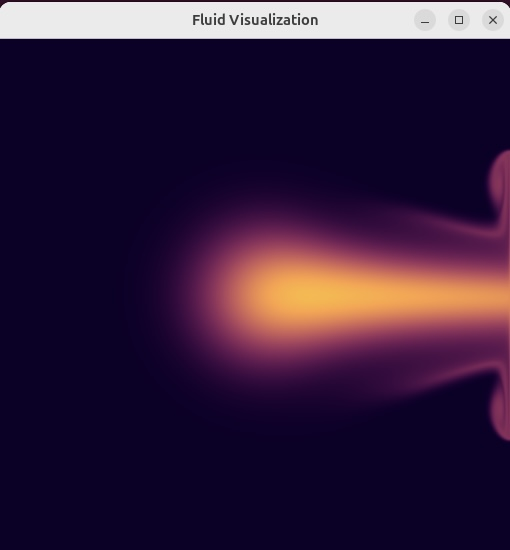
\includegraphics[width=0.78\textwidth]{IMG_9395.jpg}
\caption{Demo screenshot of dye visualization at $512 \times 512$ (command above).}
\label{fig:demo}
\end{figure}

\section{Conclusion}
We successfully reproduced the core GPU Gems Chapter 38 fluid simulation workflow with a correctness-first CPU/GPU comparison, measurable GPU acceleration, and an interactive dye-based demo. The project demonstrates that parallel grid updates on CUDA can deliver real-time behavior while maintaining numerical agreement with a CPU reference implementation.

\section{Tasks of Each Member}
\begin{itemize}
    \item \textbf{林哲安}: fluid model and solver, GPU kernel implementation.
    \item \textbf{許書瑋}: interaction, visualization, testing, and report integration.
\end{itemize}

\begin{thebibliography}{9}
\bibitem{gpugems38}
Mark J. Harris. \textit{Fast Fluid Dynamics Simulation on the GPU}. In GPU Gems, Chapter 38. NVIDIA.

\bibitem{stam}
Jos Stam. \textit{Stable Fluids}. Proceedings of SIGGRAPH, 1999.
\end{thebibliography}

\end{document}
